\documentclass[a4paper,12pt,final]{article}
% Pour une impression recto verso, utilisez plutôt ce documentclass :
%\documentclass[a4paper,11pt,twoside,final]{article}

\usepackage[english,francais]{babel}
\usepackage[utf8]{inputenc}
\usepackage[T1]{fontenc}
\usepackage[pdftex]{graphicx}
\usepackage{setspace}
\usepackage{hyperref}
\usepackage[french]{varioref}
\usepackage[top=3cm, bottom=2.8cm, left=2cm, right=2cm]{geometry}
%\usepackage{a4wide}
 \usepackage{textcomp}
\usepackage{amsmath}
\usepackage{listings}
\usepackage{color}

\definecolor{mygreen}{rgb}{0,0.6,0}
\definecolor{mygray}{rgb}{0.5,0.5,0.5}
\definecolor{mymauve}{rgb}{0.58,0,0.82}

\lstset{ %
  backgroundcolor=\color{white},   % choose the background color; you must add \usepackage{color} or \usepackage{xcolor}
  %basicstyle=\footnotesize,        % the size of the fonts that are used for the code
  breakatwhitespace=true,         % sets if automatic breaks should only happen at whitespace
  breaklines=false,                 % sets automatic line breaking
  captionpos=b,                    % sets the caption-position to bottom
  commentstyle=\color{mygreen},    % comment style
  extendedchars=true,              % lets you use non-ASCII characters; for 8-bits encodings only, does not work with UTF-8
  frame=single,                    % adds a frame around the code
  keepspaces=false,                 % keeps spaces in text, useful for keeping indentation of code (possibly needs columns=flexible)
  keywordstyle=\color{blue},       % keyword style
  language=SQL,                 % the language of the code
  morekeywords={*,...},            % if you want to add more keywords to the set
  numbers=none,                    % where to put the line-numbers; possible values are (none, left, right)
  numbersep=5pt,                   % how far the line-numbers are from the code
  numberstyle=\tiny\color{mygray}, % the style that is used for the line-numbers
  rulecolor=\color{black},         % if not set, the frame-color may be changed on line-breaks within not-black text (e.g. comments (green here))
  stringstyle=\color{mymauve},     % string literal style
  tabsize=2,                       % sets default tabsize to 2 spaces
}

\lstset{literate=
  {á}{{\'a}}1 {é}{{\'e}}1 {í}{{\'i}}1 {ó}{{\'o}}1 {ú}{{\'u}}1
  {Á}{{\'A}}1 {É}{{\'E}}1 {Í}{{\'I}}1 {Ó}{{\'O}}1 {Ú}{{\'U}}1
  {à}{{\`a}}1 {è}{{\`e}}1 {ì}{{\`i}}1 {ò}{{\`o}}1 {ù}{{\`u}}1
  {À}{{\`A}}1 {È}{{\'E}}1 {Ì}{{\`I}}1 {Ò}{{\`O}}1 {Ù}{{\`U}}1
  {ä}{{\"a}}1 {ë}{{\"e}}1 {ï}{{\"i}}1 {ö}{{\"o}}1 {ü}{{\"u}}1
  {Ä}{{\"A}}1 {Ë}{{\"E}}1 {Ï}{{\"I}}1 {Ö}{{\"O}}1 {Ü}{{\"U}}1
  {â}{{\^a}}1 {ê}{{\^e}}1 {î}{{\^i}}1 {ô}{{\^o}}1 {û}{{\^u}}1
  {Â}{{\^A}}1 {Ê}{{\^E}}1 {Î}{{\^I}}1 {Ô}{{\^O}}1 {Û}{{\^U}}1
  {œ}{{\oe}}1 {Œ}{{\OE}}1 {æ}{{\ae}}1 {Æ}{{\AE}}1 {ß}{{\ss}}1
  {ç}{{\c c}}1 {Ç}{{\c C}}1 {ø}{{\o}}1 {å}{{\r a}}1 {Å}{{\r A}}1
  {€}{{\EUR}}1 {£}{{\pounds}}1
}


\usepackage[final]{pdfpages}
\makeatletter
\renewcommand%
{\subsection}{\@startsection{subsection}{2}{10mm}
{-\baselineskip}{0.25\baselineskip}%
{\bf\large\slshape}}%
\makeatother

\makeatletter
\renewcommand%
{\subsubsection}{\@startsection{subsubsection}{2}{20mm}
{-\baselineskip}{0.25\baselineskip}%
{\normalfont\large\slshape}}%normalsize
\makeatother

\newcommand{\reporttitle}{Lab 5 :  Introduction to Q-Learning}     % Titre
\newcommand{\reportauthor}{Arnaud \textsc{Pecoraro}} % Auteur
\newcommand{\reportsubject}{TDDC17 Artificial Intelligence} % Sujet
\newcommand{\HRule}{\rule{\linewidth}{0.5mm}}
\setlength{\parskip}{1ex} % Espace entre les paragraphes

\hypersetup{
    pdftitle={\reporttitle},%
    pdfauthor={\reportauthor},%
    pdfsubject={\reportsubject},%
    pdfkeywords= {lab1, agents, intelligent}
}
\usepackage{listings}
\usepackage{color}

\definecolor{dkgreen}{rgb}{0,0.6,0}
\definecolor{gray}{rgb}{0.5,0.5,0.5}
\definecolor{mauve}{rgb}{0.58,0,0.82}

\lstset{frame=tb,
  language=Java,
    aboveskip=3mm,
  belowskip=3mm,
    showstringspaces=false,
  columns=flexible,
    basicstyle={\small\ttfamily},
  numbers=none,
    numberstyle=\tiny\color{gray},
  keywordstyle=\color{blue},
    commentstyle=\color{dkgreen},
  stringstyle=\color{mauve},
    breaklines=false,
  breakatwhitespace=false,
    tabsize=3
}
\begin{document}
  \begin{titlepage}
\thispagestyle{empty}
\begin{center}

\begin{minipage}[t]{0.48\textwidth}
  \begin{flushleft}
    
\includegraphics [width=48mm]{images/logo-univ.jpg} \\[0.5cm]

  \end{flushleft}
\end{minipage}
\begin{minipage}[t]{0.48\textwidth}
  \begin{flushright}

  \end{flushright}
\end{minipage} \\[1.0cm] %1.5

\vspace{5.3cm}

\textsc{\Large \reportsubject :}\\[2cm]

\HRule \\[0.4cm]
{\Large \bfseries \reporttitle}\\[0.4cm]
\HRule \\[1.5cm]

\vspace{1.5cm}

%\includegraphics [width=80mm]{images/ascii_art2.png} \\[0.5cm]
\vspace{4.5cm}
\begin{minipage}[t]{0.30\textwidth}
  \begin{flushleft} \normalsize
     ~Arnaud \textsc{Pecoraro} \\
 \end{flushleft}
\end{minipage}
\begin{minipage}[t]{0.6\textwidth}
  \begin{flushright} \normalsize

    %~Arnaud \textsc{Pecoraro} \\
  \end{flushright}
\end{minipage}

\vfill
\vspace*{0.440cm}
{\large October 2015 }

\end{center}
\end{titlepage}

  \cleardoublepage
  %\section*{Introduction} % Pas de numérotation
\addcontentsline{toc}{section}{Introduction} % Ajout dans la table des matières
    \thispagestyle{empty}
 \setcounter{page}{1}
\vspace{2cm}

  %\tableofcontents
  %\sloppy
  %\cleardoublepage
  \cleardoublepage
  \section*{Task 1 : Writing Domain and Problem}
\thispagestyle{empty}

The aim of this fourth lab is to learn how to model a problem that can be
solved with automatic solvers called planners, using a formal language : PDDL.

Different domains alternatives are suggested. I have chosen to implement the AI
classic Shakey's World.

Shakey is a robot with two grippers that is moving in a set of rooms, connected
by doors. Each room contains a lightswitch which can be on or off but may also
contain big boxes or smaller objects.

The lab page defines the following constraints :
\begin{itemize}
  \item Shakey can carry small objects, but only two at a time because he has
  only two grippers.
  \item For Shakey to be able to find a small object in a room, the light must
  be on in that room.
  \item Shakey can not carry boxes, but can push them around. Boxes can only be
  pushed through wide doors, not narrow ones.
  \item To switch the light in a room on or off Shakey must climb onto a box
  that is positioned below the switch (otherwise he can not reach the switch).
  This may in turn require moving the box into position, possibly from another
  room.
\end{itemize}

\begin{center}
  \begin{verbatim}
  -------------------------------------------------------------------------
  |                       |                       |                       |
  |                       |                       |                       |
  |       light switch 1 -|- light switch2        |- light switch3        |
  |                       |                       |                       |
  |       ---             |                     door2                     |
  |       | |           door1      shakey         |                       |
  |       ---           (wide)                    |                       |
  |       box             |                       |                       |
  |                       |                     door3                     |
  |                       |                     (wide)                    |
  |        room1          |        room2          |         room3         |
  -------------------------------------------------------------------------
  \end{verbatim}
  SRI Shakey's World
\end{center}

The following actions have been implemented in the domain definition file :
move, push, climb, descend, turnon and pickup and drop.

A few assumptions have been made :
\begin{itemize}
  \item Doors are either opened wide or narrow, it is not possible to change the
opening.
  \item Shakey pushing a box from a room to another imply Shakey also being in
the destination room.
  \item When Shakey is on a box, he can only turn a light on, he has to reach
the ground before being able to move.
\end{itemize}

Please refer to the code and comments for more details regarding the
implementation.

\newpage
\thispagestyle{empty}
\subsection*{Testing the domain with a simple problem}

The example below is very simple problem just to test the domain.
Shakey is in room-1 and must bring the ball from room-1 to room-3 and then
go back to room-1. A climbable box is in room-1.

The goal is defined as follow :
\begin{verbatim}
(:goal (and(in ball room-3) (in shakey room-1 )))
\end{verbatim}

Using \textit{vhpop} planner on this simple problem we get the following
solution :

\begin{figure}[h]
    \centering
      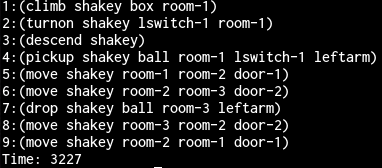
\includegraphics[width=0.50\linewidth]{./images/prob0_seq.png}
    \caption{Actions sequence using vhpop}
\end{figure}

\section*{Task 2 : Problems and performance comparison}
\thispagestyle{empty}
In this part we are going to test and compare the different planners on a range
of problems with increasing difficulty.

\subsection*{Identifying parameters}
In order to create this range of problem, we first have to identify the
parameters that can be modified to scale up the difficulty.

\begin{itemize}
  \item World dimensions : the default domain (see page 1) is composed of only
three rooms. If we add more rooms or change the disposition to a grid of (n,m)
rooms, the complexity increases rapidly.
  \item The number of objects : The difficulty increases if we add more balls
to carry to different places. If we limit the number of climbable boxes to 1,
forcing Shakey to move to the box, then push it to the switch location, and so
on...
  \item The initial state : If the initial state contains already achieved goal
conditions, the complexity is reduced.
\end{itemize}

We are going to increase the number of balls and the world dimension.

\newpage
The world dimension will be enlarged into a 3 by 3 room grid in the last
problems.
\thispagestyle{empty}
\begin{center}
  \begin{verbatim}
  -------------------------------------------------------------------------
  |                       |                       |                       |
  |       light switch 1 -|- light switch2        |- light switch3        |
  |       ---             |                     door2                     |
  |       | |           door1      shakey         |                       |
  |       ---           (wide)                    |                       |
  |       box             |                       |                       |
  |                       |                     door3                     |
  |                       |                     (wide)                    |
  |        room1          |        room2          |         room3         |
  -------door4(wide)---------------------------------------door5-----------
  |                       |                       |                       |
  |       light switch4  -|- light switch5        |- light switch6        |
  |                       |                       |                       |
  |                     door6                     |                       |
  |                     (wide)                    |                       |
  |                       |                     door7                     |
  |                       |                     (wide)                    |
  |        room4          |        room5          |         room6         |
  --------------------------------door8(wide)-------------door9------------
  |                       |                       |                       |
  |       light switch7  -|- light switch8        |- light switch9        |
  |                       |                       |                       |
  |                     door10                    |                       |
  |                     (wide)                    |                       |
  |                       |                     door11                    |
  |                       |                     (wide)                    |
  |        room7          |        room8          |         room9         |
  -------------------------------------------------------------------------
  \end{verbatim}
  SRI Shakey's World 9 rooms
\end{center}

%\newpage
\thispagestyle{empty}
\subsection*{Problems}

\textit{Here are just the relevant inforations to understand the problems.
For the complete description, please refer to the Shakey\_probX.pddl files.}
\begin{itemize}
  \item \textit{Shakey\_prob1.pddl} : 3 rooms, 3 balls
  \vspace*{1em}
  \begin{verbatim}
    (:init (in box room-2) (in ball-1 room-1) (in ball-2 room-2)
      (in ball-3 room-2) (in shakey room-1))

    (:goal (and(in ball-1 room-3)
      (in ball-2 room-1) (in ball-3 room-3)(in shakey room-3)))
  \end{verbatim}
  \item \textit{Shakey\_prob2.pddl} : 3 rooms, 6 balls
  \vspace*{1em}
  \begin{verbatim}
    (:init (in box room-2) (in ball-1 room-1)
      (in ball-2 room-2) (in ball-3 room-2) (in ball-4 room-1)
      (in ball-5 room-2) (in ball-6 room-3) (in shakey room-1))

    (:goal (and(in ball-1 room-3)
      (in ball-2 room-1) (in ball-3 room-3)(in ball-4 room-3)
      (in ball-5 room-1) (in ball-6 room-1)(in shakey room-3)))
  \end{verbatim}
  \thispagestyle{empty}
  \item \textit{Shakey\_prob3.pddl} : 3 rooms, 12 balls
  \vspace*{1em}
  \begin{verbatim}
    (:init (in box room-2) (in ball-1 room-1)
      (in ball-2 room-2) (in ball-3 room-2) (in ball-4 room-1)
      (in ball-5 room-2) (in ball-6 room-3) (in ball-7 room-1)
      (in ball-8 room-2) (in ball-9 room-2) (in ball-10 room-1)
      (in ball-11 room-2) (in ball-12 room-3) (in shakey room-1))

    (:goal (and(in ball-1 room-3)
      (in ball-2 room-1) (in ball-3 room-3)(in ball-4 room-3)
      (in ball-5 room-1) (in ball-6 room-1)(in ball-7 room-3)
      (in ball-8 room-1) (in ball-9 room-3)(in ball-10 room-2)
      (in ball-11 room-3) (in ball-12 room-1)(in shakey room-3)))
  \end{verbatim}
  \item \textit{Shakey\_prob4.pddl} : 9 rooms, 1 ball
  \vspace*{1em}
  \begin{verbatim}
    (:init (in box room-1) (in ball-1 room-3) (in shakey room-2))

    (:goal (in ball-1 room-9))
  \end{verbatim}
  \item \textit{Shakey\_prob5.pddl} : 9 rooms, 3 balls
  \vspace*{1em}
  \begin{verbatim}
    (:init (in box room-1) (in ball-1 room-3) (in ball-2 room-6)
      (in ball-3 room-9) (in shakey room-2))

    (:goal (and(in ball-1 room-9) (in ball-3 room-1) (in ball-2 room-7)))
  \end{verbatim}
  \item \textit{Shakey\_prob6.pddl} : 9 rooms, 6 balls
  \vspace*{1em}
  \begin{verbatim}
    (:init (in box room-1) (in ball-1 room-3) (in ball-2 room-6)
      (in ball-3 room-9) (in ball-4 room-3) (in ball-5 room-3)
      (in ball-6 room-9) (in shakey room-2) (movable shakey))

    (:goal
      (and(in ball-1 room-9) (in ball-3 room-1) (in ball-2 room-7)
      (in ball-4 room-9) (in ball-5 room-7) (in ball-6 room-2)))
  \end{verbatim}
\end{itemize}
\newpage
\subsection*{Results}
\thispagestyle{empty}
\textit{Test protocol : all tests have been done in the same conditions, on
the same computer (Liu server, accessed via thinlinc). A time limit of 3600s
has been choosen. If no solution has been found, the test failed.}
\thispagestyle{empty}

The results on this problem set are presented in \textit{Figure 2}.

\begin{figure}[h]
    \centering
    \begin{tabular}{cc}
      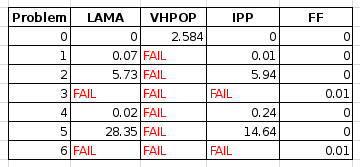
\includegraphics[width=.49\linewidth,scale=1]{./images/tab1.png} &
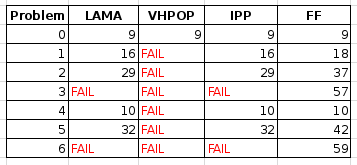
\includegraphics[width=.49\linewidth, scale=1.5]{./images/tab2.png} \\
      (a) & (b)
    \end{tabular}
    \caption{Running time in seconds (a) and path cost (b)}
\end{figure}

Firstly, we noticed that \textit{VHPOP} failed in every problem but problem 0.
In fact
the process is automatically killed before reaching the choosen time limit.

As far as speed is concerned, \textit{FF} is a clear winner. Every planning
problem is almost solved instantly. However, except in problem 0 and 4, the
solution is never optimal.

On the other hand \textit{LAMA} and \textit{IPP} always find the least-cost
solution but the running time much longer as the problem become more difficult.

\textit{Note : in Figure 2, when LAMA "fails", it means that the algorithms did
not finish the exhausted search in time and therefore may not have found the
optimal solution yet. It did not mean that no solution where found.}

\subsection*{Adding more problems to the sets}

In order to better understand the influence of each parameters, I have added
three more problems.

\begin{itemize}
  \item \textit{Shakey\_prob2.5.pddl} : 3 rooms, 8 balls
  \vspace*{1em}
  \begin{verbatim}
    (:init (in box room-2) (in ball-1 room-1) (in ball-2 room-2)
      (in ball-3 room-2) (in ball-4 room-1) (in ball-8 room-2)
      (in ball-10 room-1)(in ball-11 room-2) (in ball-12 room-3)
      (in shakey room-1))

      (:goal (and(in ball-1 room-3) (in ball-2 room-1) (in ball-3 room-3)
        (in ball-4 room-3) (in ball-8 room-1)(in ball-10 room-2)
        (in ball-11 room-3) (in ball-12 room-1)(in shakey room-3)))

  \end{verbatim}
  \item \textit{Shakey\_prob4.5.pddl} : 9 rooms, 2 balls
  \vspace*{1em}
  \begin{verbatim}
    (:init  (in box room-1)(in ball-1 room-3)(in ball-2 room-6)
      (in ball-3 room-9) (in shakey room-2)

    (:goal (and(in ball-1 room-9) (in ball-2 room-7)))
  \end{verbatim}
  \thispagestyle{empty}
  \item \textit{Shakey\_prob5.5.pddl} : 9 rooms, 4 balls
  \vspace*{1em}
  \begin{verbatim}
    (:init  (in box room-1) (in ball-1 room-3) (in ball-3 room-9)
      (in ball-5 room-3) (in ball-6 room-9) (in shakey room-2)

      (:goal (and(in ball-1 room-9) (in ball-3 room-1)
        (in ball-5 room-7) (in ball-6 room-2)))
    \end{verbatim}
\end{itemize}

Results are presented in the \textit{Figure 3} below. Given the previous tests,
\textit{VHPOP} has not been used. The first solution returned by \textit{LAMA}
and its running time have been added to the comparison.

\begin{figure}[h]
    \centering
    \begin{tabular}{cc}
      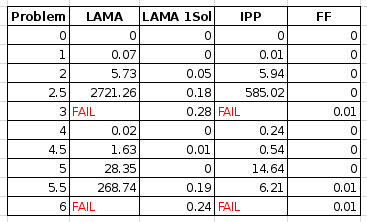
\includegraphics[width=.49\linewidth,scale=1]{./images/tab3.png} &
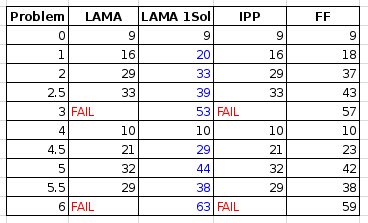
\includegraphics[width=.49\linewidth, scale=1.5]{./images/tab4.png} \\
      (a) & (b)
    \end{tabular}
    \caption{Running time in seconds (a) and path cost (b)}
\end{figure}


We notice with problems 2.5, 5.5, and 6 that adding more balls
increases the difficulty drastically. A clear example is the difference
between problem 5 and 5.5.

An interesting fact, is that except in the simpliests problems, the first
solution returned by \textit{LAMA} is never optimal. It is not as fast as
\textit{FF} and in this range of problem its optimality is comparable, sometimes
better, sometimes worst see \textit{Figure 3b} and \textit{Figure 4}.

In this test set, the best solution for optimality would be \textit{IPP}, it
always find the optimal solution and sometimes way faster than \textit{LAMA}'s
exhaustive search, see problem 5.5 for example.

On the other hand, if speed is what matter the most, \textit{FF} seems to be
the best tradeoff.

\newpage
\thispagestyle{empty}
\begin{figure}[h]
    \centering
      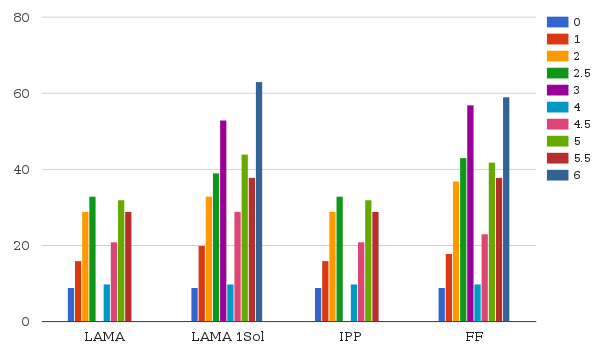
\includegraphics[width=.65\linewidth,scale=1]{./images/graph.png}
    \caption{Path cost comparison graph}
\end{figure}

As a conclusion, we notice that as planning problem grows larger, they
cannot be solved optimaly in reasonable time. Here this is the case with problem
6.

  \cleardoublepage
  %\include{partie2}
  %\cleardoublepage
  %\include{partie3}
  %\cleardoublepage
  %\section*{Conclusion}
\addcontentsline{toc}{section}{Conclusion}
\vspace{2cm}

  %\cleardoublepage
\end{document}
